\documentclass[tikz,border=2pt]{standalone}
\usepackage{amsmath,amssymb}
\usepackage{tikz}
\usetikzlibrary{arrows.meta}

\begin{document}
% Right-hand-side range for the finishing constraint 2 x_s + x_t <= b_1: as b_1 moves, the
% optimal corner slides along x_s + x_t = 80; the same two constraints stay binding for
% 80 <= b_1 <= 120, beyond which another constraint takes over.
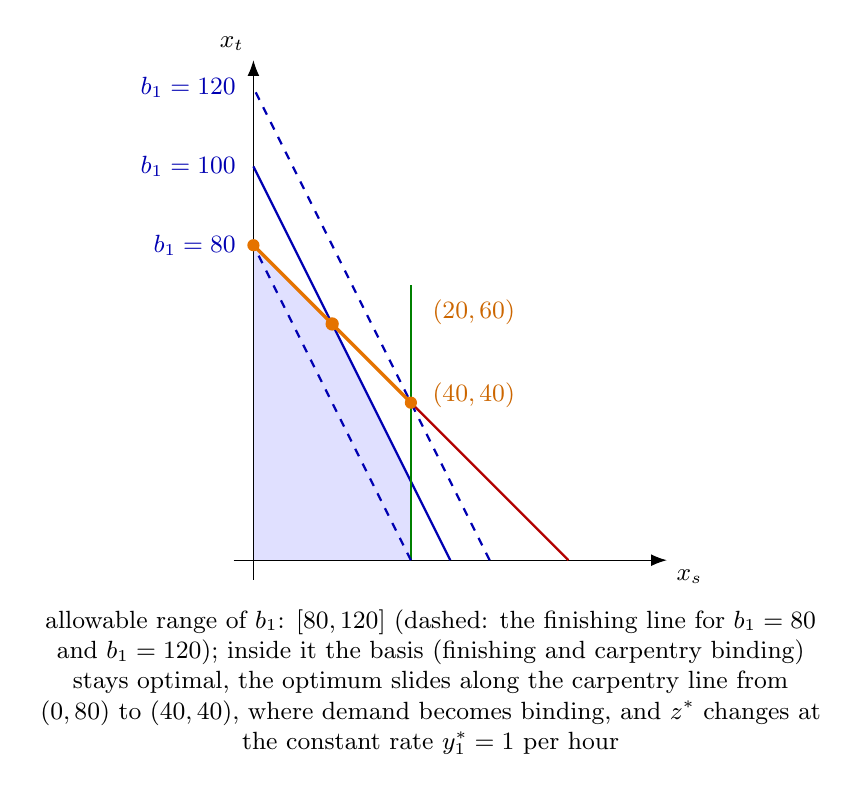
\begin{tikzpicture}[x=0.05cm, y=0.05cm, every node/.style={font=\small}, >={Latex[length=2mm]}]
	\fill[blue!12] (0,0) -- (40,0) -- (40,20) -- (20,60) -- (0,80) -- cycle;
	\draw[->] (-5,0) -- (105,0) node[below right] {$x_s$};
	\draw[->] (0,-5) -- (0,127) node[above left] {$x_t$};
	\draw[blue!70!black, thick] (50,0) -- (0,100);
	\draw[red!70!black, thick] (80,0) -- (0,80);
	\draw[green!50!black, thick] (40,0) -- (40,70);
	\draw[blue!70!black, thick, dashed] (40,0) -- (0,80);
	\draw[blue!70!black, thick, dashed] (60,0) -- (0,120);
	\node[blue!70!black, font=\small, anchor=east] at (-2,120) {$b_1=120$};
	\node[blue!70!black, font=\small, anchor=east] at (-2,100) {$b_1=100$};
	\node[blue!70!black, font=\small, anchor=east] at (-2,80) {$b_1=80$};
	\draw[orange!90!black, very thick] (0,80) -- (40,40);
	\fill[orange!90!black] (20,60) circle (2.4pt);
	\fill[orange!90!black] (0,80) circle (2.2pt);
	\fill[orange!90!black] (40,40) circle (2.2pt);
	\node[orange!80!black, font=\small, anchor=west] at (43,63) {$(20,60)$};
	\node[orange!80!black, font=\small, anchor=west] at (43,42) {$(40,40)$};
	\node[anchor=north, align=flush center, text width=10cm] at (45,-10) {allowable range of $b_1$: $[80,120]$ (dashed: the finishing line for $b_1=80$ and $b_1=120$); inside it the basis (finishing and carpentry binding) stays optimal, the optimum slides along the carpentry line from $(0,80)$ to $(40,40)$, where demand becomes binding, and $z^\ast$ changes at the constant rate $y_1^\ast=1$ per hour};
\end{tikzpicture}
\end{document}
